\documentclass[11pt]{article}
\usepackage{../../styles/activity}

\usepackage{xr}
\externaldocument{0-MR}

\lhead{}
%\chead{\textbf{\Large{\hspace{0pt}Beginning Activities for Section~6.2}}\\\hspace{0pt}\emph{Mathematical Reasoning: Writing and Proof}}
\bahead{6.2}
\rhead{}
\lfoot{}
\rfoot{}
\cfoot{\hspace{0pt}\scalebox{0.4}{
\includegraphics{cc-by-nc-sa.eps}}}

\begin{document}

\subsection*{Beginning Activity 1 (The Number of Diagonals of a Polygon)}
\begin{enumerate}
\item A triangle does not have any diagonals.  A square and a quadrilateral each have two diagonals.
%\begin{multicols}{2}
%The diagram to the right shows the 9 diagonals for a hexagon. \\
%\scalebox{0.2}{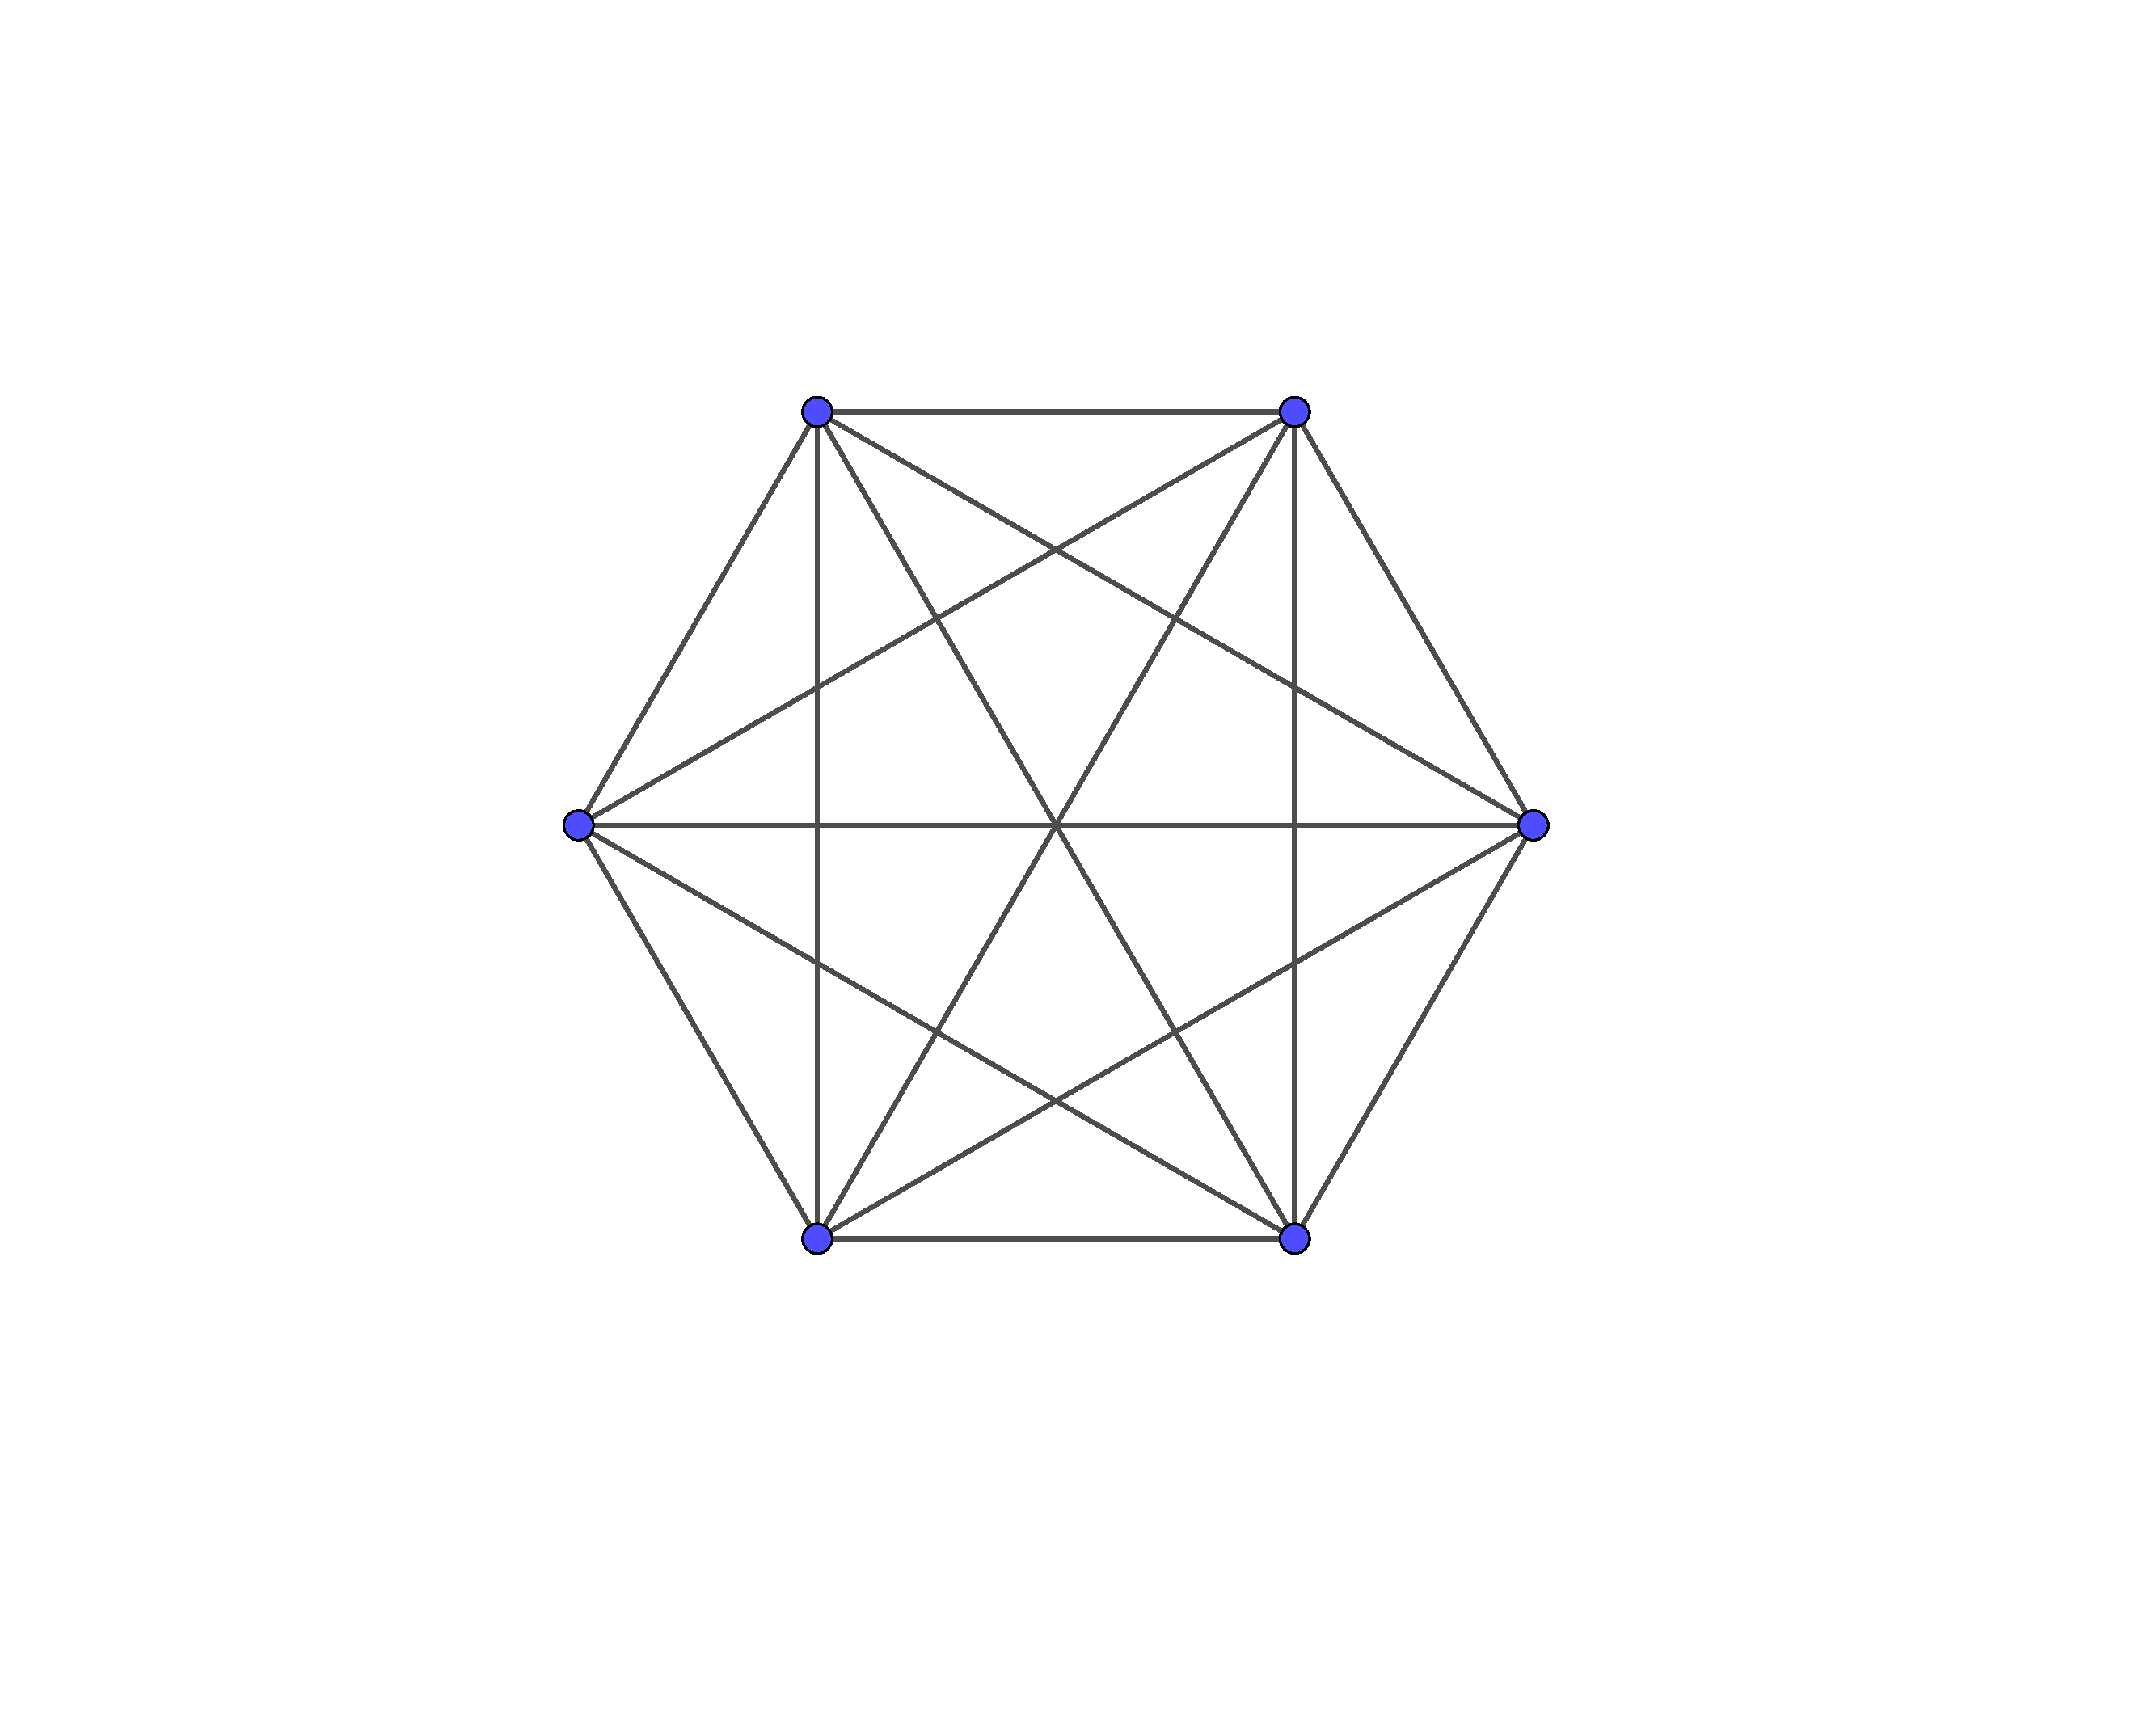
\includegraphics{hexagon-diagonals.eps}}
%\end{multicols}
\begin{minipage}{3in}
The diagram to the right shows the 9 diagonals for a hexagon.
\one
\end{minipage}
\begin{minipage}{2in}
\begin{center}
\scalebox{0.17}{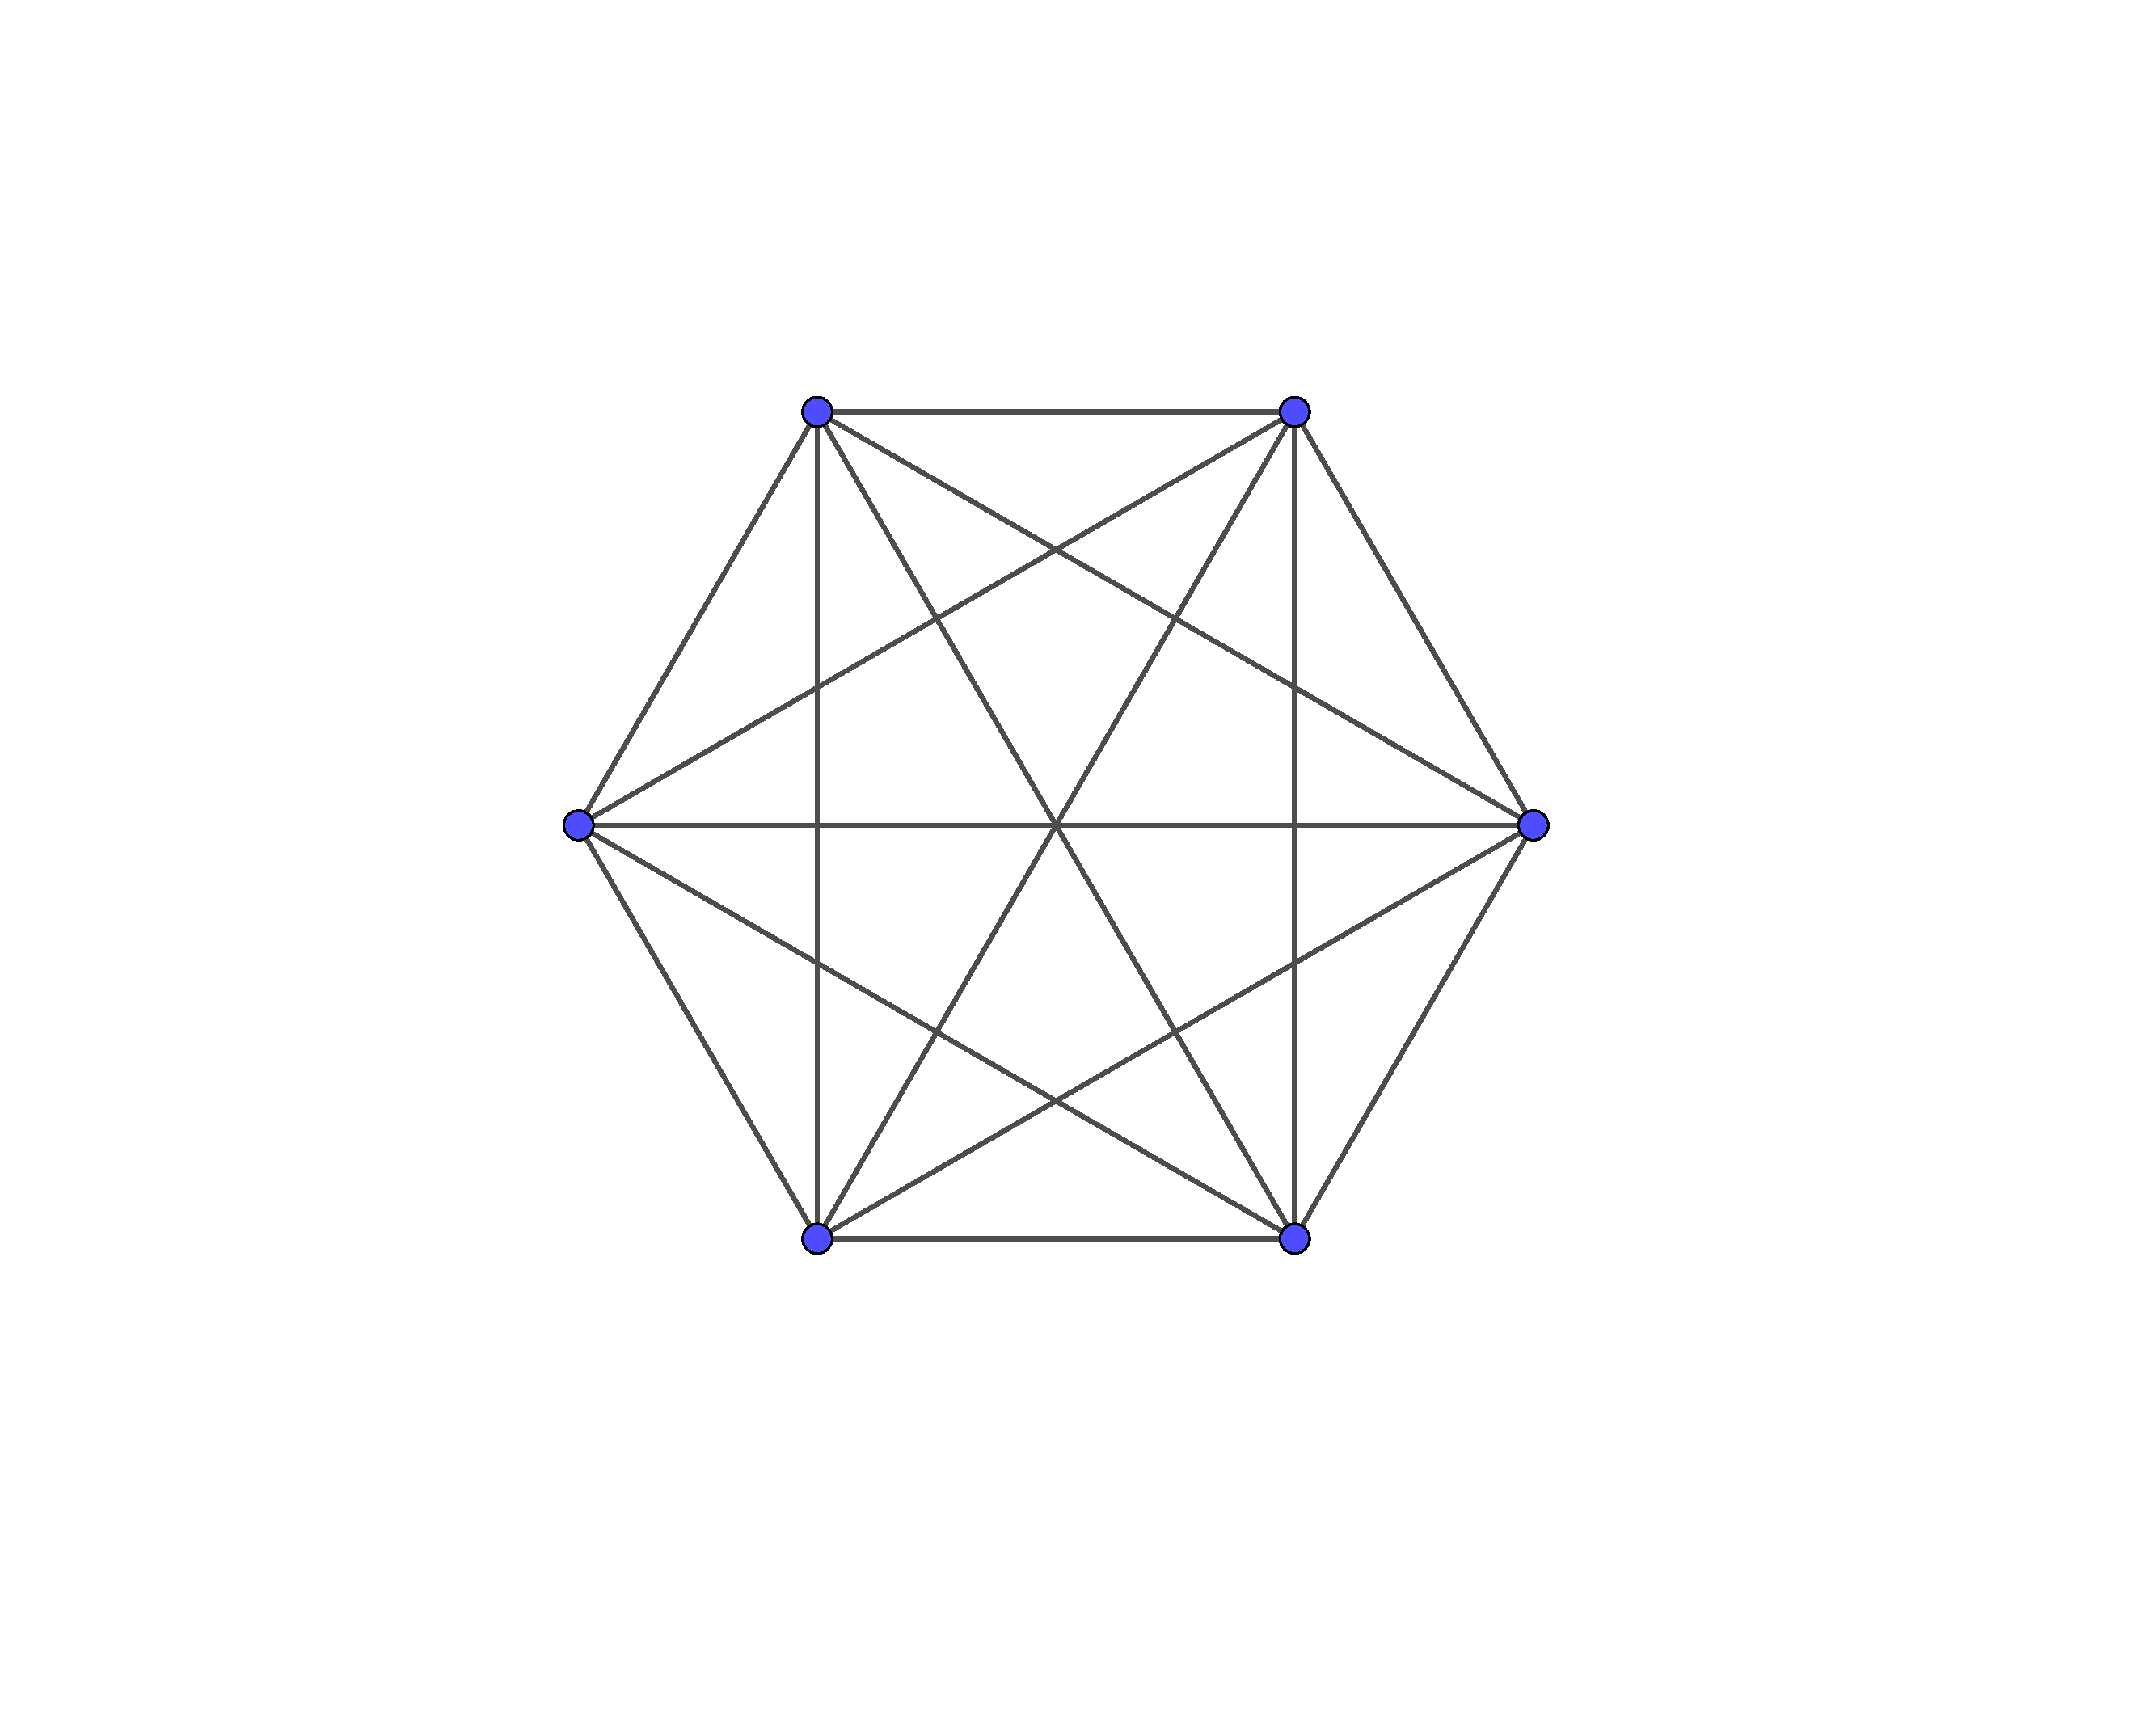
\includegraphics{hexagon-diagonals.eps}}
\end{center}
\end{minipage}


\item \begin{multicols}{2}
\begin{tabular}[t]{| c | c | c | c | c |} \cline{1-2} \cline{4-5}
$n$ &  $d ( n )$ &  & $n$ & $d ( n )$   \\ \cline{1-2} \cline{4-5}
3  &  0  &  & 7  &  14  \\ \cline{1-2} \cline{4-5}
4  &  2  &  & 8  &  20  \\ \cline{1-2} \cline{4-5}
5  &  5  &  & 9  &  27  \\ \cline{1-2} \cline{4-5}
6  &  9  &  & 10 &  35  \\ \cline{1-2} \cline{4-5}
\end{tabular}

\item \begin{tabular}[t]{| c | c | c | c | c |} \cline{1-2} \cline{4-5}
  $x$ &  $f ( x )$ &  & $x$ & $f ( x )$   \\ \cline{1-2} \cline{4-5}
0  &  0  &  & 5  &  5  \\ \cline{1-2} \cline{4-5}
1  &  -1  &  & 6  &  9  \\ \cline{1-2} \cline{4-5}
2  &  -1  &  & 7  &  14  \\ \cline{1-2} \cline{4-5}
3  &  0  &  & 8  &  20  \\ \cline{1-2} \cline{4-5}
4  &  2  &  & 9  &  27  \\ \cline{1-2} \cline{4-5}
\end{tabular}
\end{multicols}

\item The outputs of the function  $f$  are determined  by a formula, and the outputs of the function  $d$  are determined by a verbal description. This does not mean the two functions are not equal.  However, the facts that the two functions have different domains and codomains would mean that these two functions are not equal.
\end{enumerate}
\hbreak



\subsection*{Beginning Activity 2 (Derivatives)}
\begin{enumerate}
\item \begin{multicols}{2}
\begin{enumerate}
\item $f'( x ) = 4x^3  - 15x^2  + 3$
\item $g'( x ) =  - 5\sin ( {5x} )$
\item $h'( x ) = \dfrac{{x( {\cos x} ) - \sin x}}{{x^2 }}$
\item $k'( x ) =  - 2xe^{ - x^2 } $
\item $r'( x ) = \left\{ \begin{gathered}  1\text{     if  }x > 0 \hfill \\   - 1\text{  if  }x < 0 \hfill \\ \end{gathered}  \right.$
\end{enumerate}
\end{multicols}
Notice that the function  $r$  is not differentiable at $x=0$  .

\item Differentiation can be thought of as a function in the sense that if a function is considered the input, then the output is the derivative of that function.  The domain of the function is the set of all differentiable real functions and the codomain is the set of all real functions.
\end{enumerate}
\hbreak




\end{document}

